% Copyright 2007 by Till Tantau
%
% This file may be distributed and/or modified
%
% 1. under the LaTeX Project Public License and/or
% 2. under the GNU Public License.
%
% See the file doc/licenses/LICENSE for more details.


\lecture[3]{Visualizing and Summarizing}{lecture-text}

\subtitle{means, medians, and plots}

\date{20 January 2015}


\begin{document}

\begin{frame}
  \maketitle
\end{frame}

% Overview of the problem:
%   different scales of data
% Measures of Center:
%   median
%   mean
%   comparison
% Boxplots:
%   quartiles
%   outliers
%   compared to histograms
% Visualizing relationships
%   categorical-categorical: stacked freqs
%   numeric-categorical: boxplots or dotplots
%   numeric-numeric: scatterplots



%%%%%
\begin{frame}{Overview}
    \begin{enumerate}
        \item Goal: describe a dataset, i.e.
        \item summarize important quantities (statistics)
        \item and visualize the data (plots)
    \end{enumerate}

    Generally, these are \alert{descriptive statistics}.
\end{frame}


%%%%%
\begin{frame}\frametitle<presentation>{Outline}
  \tableofcontents
\end{frame}


%%%%% %%%%%
\section{Measures of Center}


%%%%%
\begin{frame}{The Median}

    The \alert{median} of a collection of observations
    is
    \begin{enumerate}
        \item[$n$ odd] the middle value.
        \item[$n$ even] the average of the middle two values.
    \end{enumerate}


    \structure{Example:} Weight gain of lambs:
    \begin{center}
        \begin{tabular}{cccccc}
            11 & 13 & 19 & 2 & 10 & 1
        \end{tabular}
    \end{center}

    \pause

    \structure{``Example:''} Weight gain of baby sharks:
    \begin{center}
        \begin{tabular}{cccccc}
            11 & 13 & 190 & 2 & 10 & 1
        \end{tabular}
    \end{center}

\end{frame}


%%%%%
\begin{frame}{The Mean}

    The \alert{mean} (or ``average'') of a collection of observations is
    \begin{enumerate}
        \item the sum of the observations, divided by the number of observations:
            \[
                \bar y = \frac{ y_1 + \cdots + y_n }{ n  }
            \]
    \end{enumerate}

    \pause

    \structure{Note:} the sum of deviations from the mean are always zero.
    \[
        (y_1 - \bar y) + (y_2 - \bar y) + \cdots + (y_n - \bar y) = 0
    \]

    \pause

    \structure{Example:} Weight gain of lambs:
    \begin{center}
        \begin{tabular}{cccccc}
            11 & 13 & 19 & 2 & 10 & 1
        \end{tabular}
    \end{center}

    \pause

    \structure{``Example:''} Weight gain of baby sharks:
    \begin{center}
        \begin{tabular}{cccccc}
            11 & 13 & 190 & 2 & 10 & 1
        \end{tabular}
    \end{center}

\end{frame}


%%%%%
\begin{frame}{Robustness}

    A statistic is \alert{robust} if it doesn't change much
    even if a small number of observations change by a lot.

    \vspace{3em}

    These are ``robust to errors'' in the data.

    \vspace{3em}

    Conversely, they tend to not ``use all the data''.

\end{frame}


%%%%%
\begin{frame}{the Quartiles}

    divide the data into \emph{quarters}:
    \begin{itemize}
        \item the \alert{first quartile} is the median of the {lower half}
        \item the \alert{second quartile} is the median
        \item the \alert{third quartile} is the median of the {upper half}
    \end{itemize}

    The \alert{interquartile range} (\textbf{IQR}) is the difference between the third and the first quartiles.

    \pause

    \structure{Example:} blood pressures.
    \begin{center}
        \begin{tabular}{ccccccc}
            151 & 124 & 132 & 170 & 146 & 124 & 113
        \end{tabular}
    \end{center}

    \pause

    \structure{Example:} pulses.
    \begin{center}
        \begin{tabular}{cccccccccccc}
            62 & 64 & 68 & 70 & 70 & 74 & 74 & 76 & 76 & 78 & 78 & 80 
        \end{tabular}
    \end{center}

\end{frame}


\section{Boxplots}

%%%%%
\begin{frame}{Boxplots: the ``five-number'' summary}

    \begin{center}
        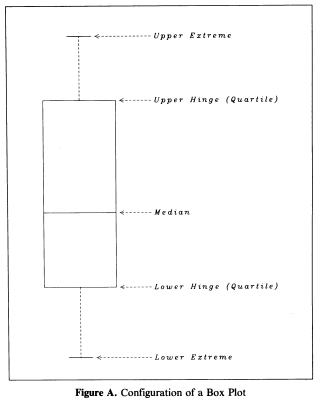
\includegraphics[height=.85\textheight]{boxplot-taxonomy.png}
        \figcaption{McGill, Tukey, \& Larson 1978}
    \end{center}

\end{frame}


%%%%%
\begin{frame}{Boxplots: modified}

    Medians and quartiles are \textbf{robust},
    but not the \alert{extremes}.

    \vspace{3em}

    We'd like the boxplot to be robust. 

    \vspace{3em}

    \structure{Solution:}
    Extend the whiskers out only to
    \[
        \text{( quartile )} \; \pm \; 1.5 \times \text{( IQR )} 
    \]

\end{frame}

%%%%%
\begin{frame}{Comparison: earthquakes}

    SoCal earthquakes in 2014, \\
    {\small from \url{http://service.scedc.caltech.edu/ftp/catalogs/SCEC_DC/2014.catalog} }

    \begin{center}
        \includegraphics<1>[width=\textwidth]{quakes-dotplot}
        \includegraphics<2>[width=\textwidth]{quakes-hist}
        \includegraphics<3>[width=\textwidth]{quakes-boxplot}
        \includegraphics<4>[width=\textwidth]{quakes-modified-boxplot}
    \end{center}

\end{frame}


%%%%% %%%%%
\section{Stacked frequency plots}

%%%%%
\begin{frame}{Absolute frequencies}
    \begin{center}
        % \begin{column}{0.5\textwidth}
            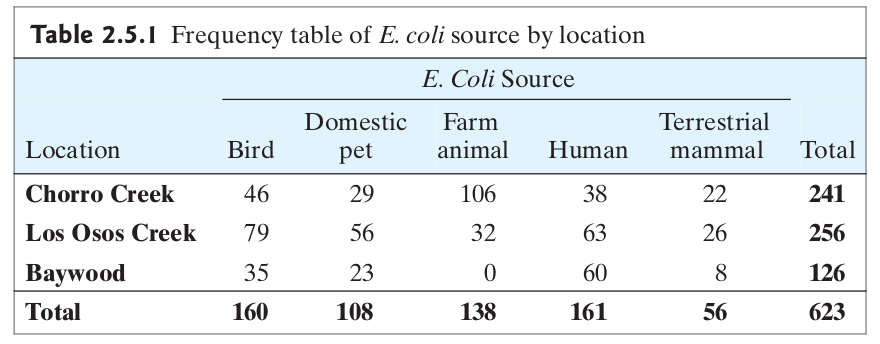
\includegraphics[width=.8\textwidth]{ecoli-counts-tab2_5_1.png}
        % \end{column}

        % \begin{column}{0.5\textwidth}
            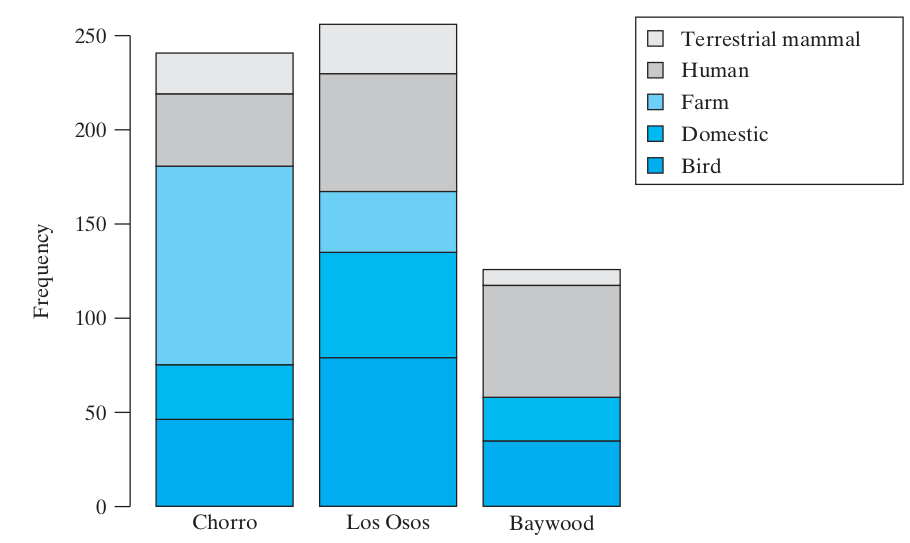
\includegraphics[width=.8\textwidth]{ecoli-counts-fig2_5_1.png}
        % \end{column}
    \end{center}
\end{frame}

%%%%%
\begin{frame}{Relative frequencies}
    \begin{center}
        % \begin{column}{0.5\textwidth}
            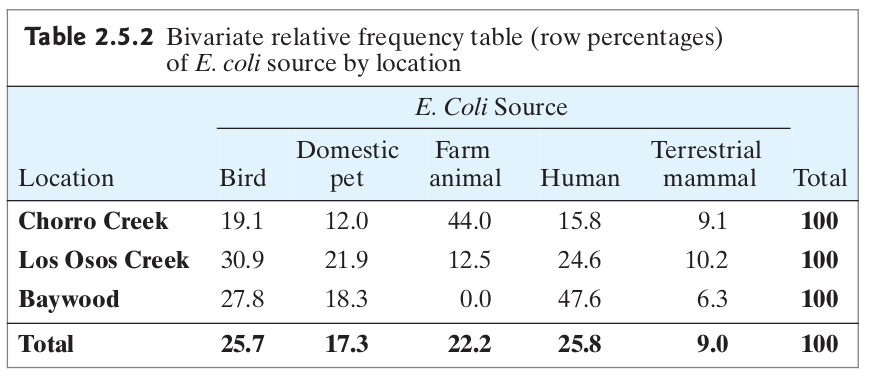
\includegraphics[width=0.8\textwidth]{ecoli-freqs-tab2_5_2.png}
        % \end{column}

        % \begin{column}{0.5\textwidth}
            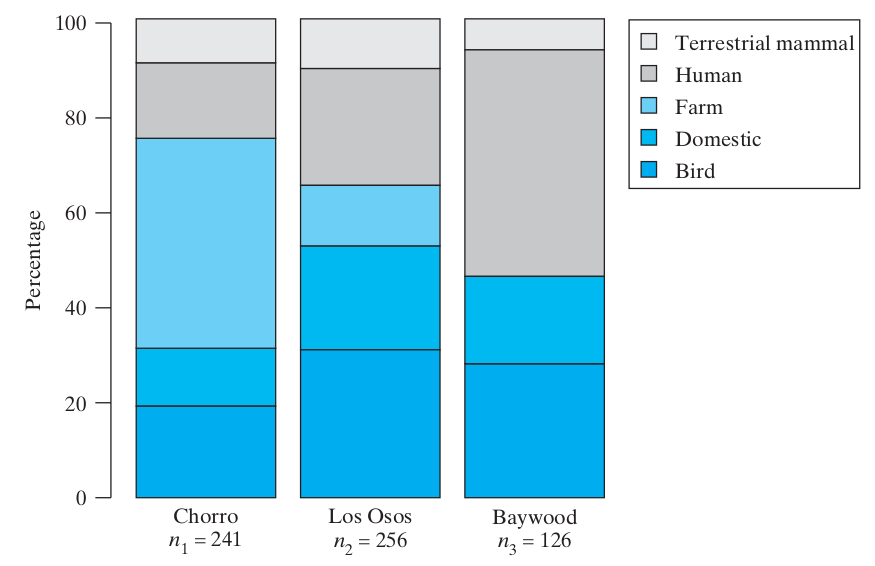
\includegraphics[width=0.8\textwidth]{ecoli-freqs-fig2_5_2.png}
        % \end{column}
    \end{center}
\end{frame}


%%%%%
\begin{frame}{What's the difference?}

    \begin{columns}
        \begin{column}{0.5\textwidth}
    \begin{center}
            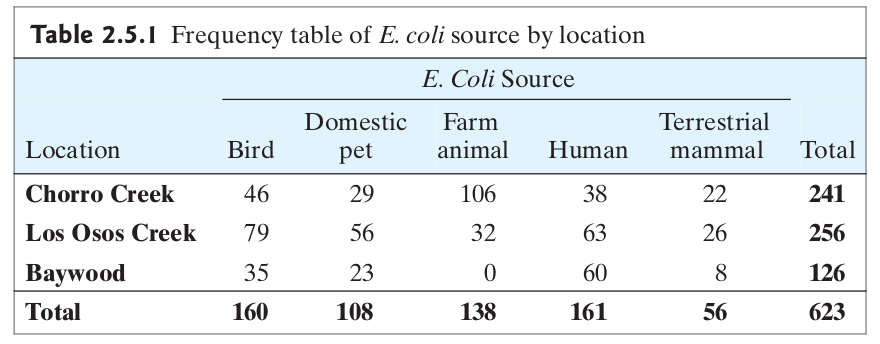
\includegraphics[width=.9\textwidth]{ecoli-counts-tab2_5_1.png}

            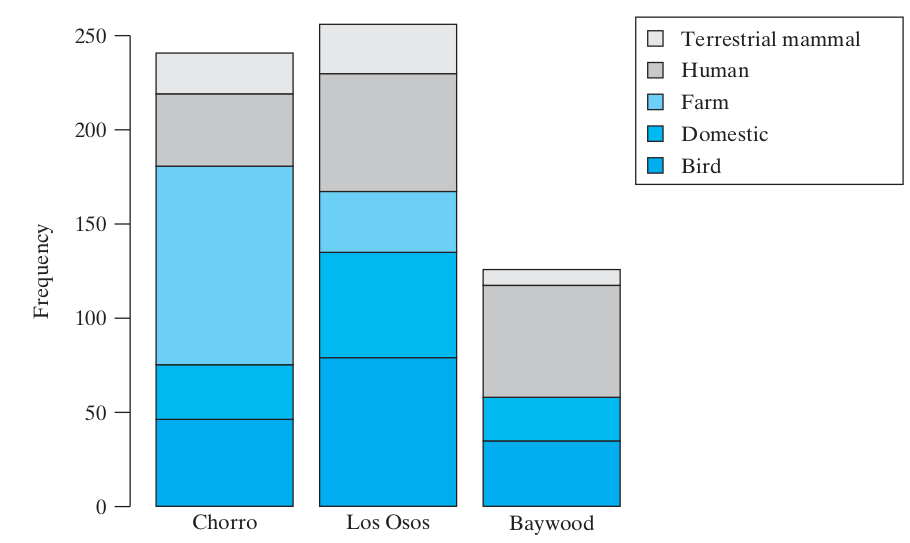
\includegraphics[width=.9\textwidth]{ecoli-counts-fig2_5_1.png}
    \end{center}
        \end{column}

        \begin{column}{0.5\textwidth}

    \begin{center}
            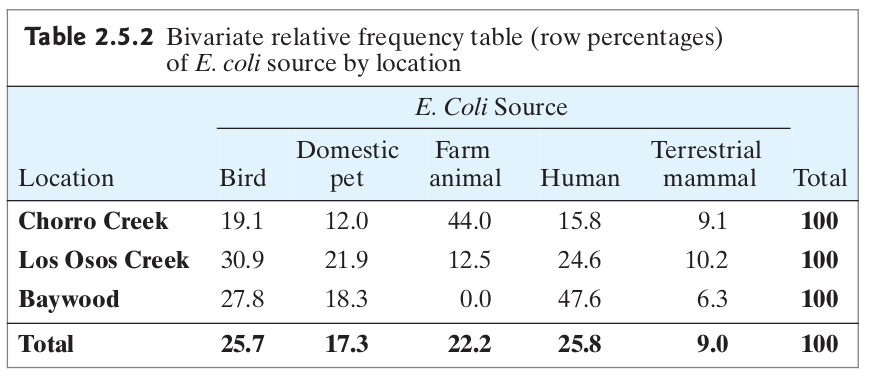
\includegraphics[width=.9\textwidth]{ecoli-freqs-tab2_5_2.png}

            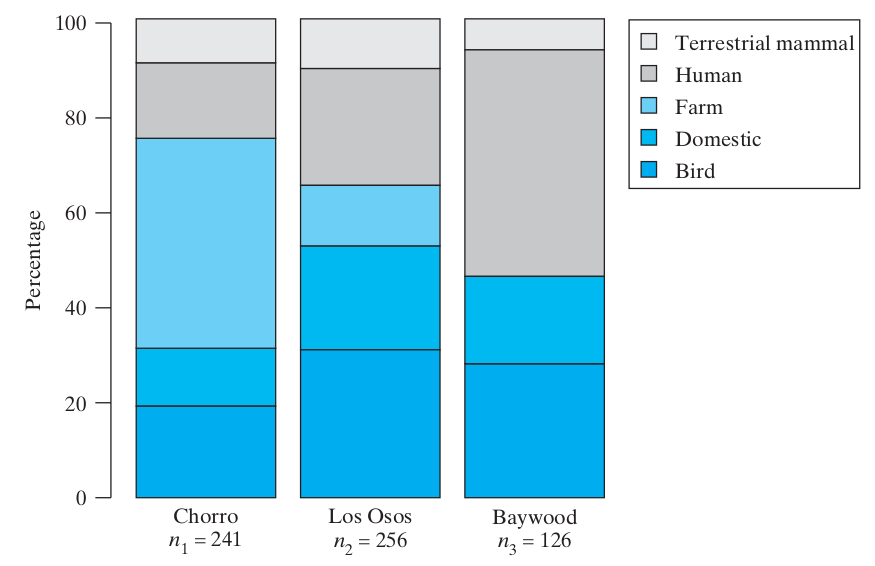
\includegraphics[width=.9\textwidth]{ecoli-freqs-fig2_5_2.png}
    \end{center}
\end{column}
\end{columns}

\end{frame}


%%%%% %%%%%
\section{Categorical-numeric relationships}

%%%%%
\begin{frame}{Boxplots, by category}

    Earthquakes, again:
    \begin{center}
        \includegraphics<1>[width=\textwidth]{quakes-category-dotplot}
        \includegraphics<2>[width=\textwidth]{quakes-category-boxplot}
    \end{center}

\end{frame}

\section<article>{Summary}
\section<presentation>*{Summary}

\begin{frame}{Summary}
  \begin{enumerate}
      \item
  \end{enumerate}
\end{frame}

% homework
\begin{frame}{Homework}
  \begin{center}

  2.3.10, 2.3.15, 2.3.16

  \vspace{2em}


  2.4.3
  

  \end{center}
\end{frame}


\end{document}
